\documentclass{article}

\usepackage{hyperref}
\usepackage{fancyhdr}
\usepackage{braket}
\usepackage{extramarks}
\usepackage{amsmath}
\usepackage{amsthm}
\usepackage{amsfonts}
\usepackage{tikz}
\usepackage[plain]{algorithm}
\usepackage{algpseudocode}
\usepackage{mathtools}
\usepackage{graphicx}
\graphicspath{ {./Images/} }

\DeclarePairedDelimiter\abs{\lvert}{\rvert}%
\DeclarePairedDelimiter\norm{\lVert}{\rVert}%

\makeatletter
\let\oldabs\abs
\def\abs{\@ifstar{\oldabs}{\oldabs*}}
%
\let\oldnorm\norm
\def\norm{\@ifstar{\oldnorm}{\oldnorm*}}
\makeatother

\newcommand*{\Value}{\frac{1}{2}x^2}%

\usetikzlibrary{automata,positioning}

%
% Basic Document Settings
%

\topmargin=-0.45in
\evensidemargin=0in
\oddsidemargin=0in
\textwidth=6.5in
\textheight=9.0in
\headsep=0.25in

\linespread{1.1}

\pagestyle{fancy}
\lhead{\hmwkAuthorName}
\chead{\hmwkClass\ (\hmwkClassInstructor\ \hmwkClassTime): \hmwkTitle}
\rhead{\firstxmark}
\lfoot{\lastxmark}
\cfoot{\thepage}

\renewcommand\headrulewidth{0.4pt}
\renewcommand\footrulewidth{0.4pt}

\setlength\parindent{0pt}

%
% Create Problem Sections
%

\newcommand{\enterProblemHeader}[1]{
    \nobreak\extramarks{}{Problem \arabic{#1} continued on next page\ldots}\nobreak{}
    \nobreak\extramarks{Problem \arabic{#1} (continued)}{Problem \arabic{#1} continued on next page\ldots}\nobreak{}
}

\newcommand{\exitProblemHeader}[1]{
    \nobreak\extramarks{Problem \arabic{#1} (continued)}{Problem \arabic{#1} continued on next page\ldots}\nobreak{}
    \stepcounter{#1}
    \nobreak\extramarks{Problem \arabic{#1}}{}\nobreak{}
}

\setcounter{secnumdepth}{0}
\newcounter{partCounter}
\newcounter{homeworkProblemCounter}
\setcounter{homeworkProblemCounter}{1}
\nobreak\extramarks{Problem \arabic{homeworkProblemCounter}}{}\nobreak{}

%
% Homework Problem Environment
%
% This environment takes an optional argument. When given, it will adjust the
% problem counter. This is useful for when the problems given for your
% assignment aren't sequential. See the last 3 problems of this template for an
% example.
%
\newenvironment{homeworkProblem}[1][-1]{
    \ifnum#1>0
        \setcounter{homeworkProblemCounter}{#1}
    \fi
    \section{Problem \arabic{homeworkProblemCounter}}
    \setcounter{partCounter}{1}
    \enterProblemHeader{homeworkProblemCounter}
}{
    \exitProblemHeader{homeworkProblemCounter}
}

%
% Homework Details
%   - Title
%   - Due date
%   - Class
%   - Section/Time
%   - Instructor
%   - Author
%

\newcommand{\hmwkTitle}{Homework\ \#10}
\newcommand{\hmwkDueDate}{April 7, 2020}
\newcommand{\hmwkClass}{Physics 926}
\newcommand{\hmwkClassTime}{}
\newcommand{\hmwkClassInstructor}{Professor Ken Bloom}
\newcommand{\hmwkAuthorName}{\textbf{Robert Tabb}}

%
% Title Page
%

\title{
    \vspace{2in}
    \textmd{\textbf{\hmwkClass:\ \hmwkTitle}}\\
    \normalsize\vspace{0.1in}\small{Due\ on\ \hmwkDueDate\ at 5pm}\\
    \vspace{0.1in}\large{\textit{\hmwkClassInstructor\ \hmwkClassTime}}
    \vspace{3in}
}

\author{\hmwkAuthorName}
\date{}

\renewcommand{\part}[1]{\textbf{\large Part \Alph{partCounter}}\stepcounter{partCounter}\\}

%
% Various Helper Commands
%

% Useful for algorithms
\newcommand{\alg}[1]{\textsc{\bfseries \footnotesize #1}}

% For derivatives
\newcommand{\deriv}[1]{\frac{\mathrm{d}}{\mathrm{d}x} (#1)}

% For partial derivatives
\newcommand{\pderiv}[2]{\frac{\partial}{\partial #1} (#2)}

% Integral dx
\newcommand{\dx}{\mathrm{d}x}

% Alias for the Solution section header
\newcommand{\solution}{\textbf{\large Solution}}

% Probability commands: Expectation, Variance, Covariance, Bias
\newcommand{\E}{\mathrm{E}}
\newcommand{\Var}{\mathrm{Var}}
\newcommand{\Cov}{\mathrm{Cov}}
\newcommand{\Bias}{\mathrm{Bias}}

\begin{document}

\maketitle
*In addition to the lecture notes, the following resources were used to better understand the material:\\
\url{https://arxiv.org/pdf/hep-ph/0401236.pdf}\\
\url{https://www.hep.phy.cam.ac.uk/~thomson/lectures/partIIIparticles/Handout12_2009.pdf}
\pagebreak

\begin{homeworkProblem}
	Show that:
	\[
		\frac{\Gamma(K_L \rightarrow \pi^-e^+\nu_e)-\Gamma(K_L \rightarrow \pi^+e^-\bar{\nu}_e))}{\Gamma(K_L \rightarrow \pi^-e^+\nu_e)+\Gamma(K_L \rightarrow \pi^+e^-\bar{\nu}_e))} = 2Re(\epsilon)
	\]
	to first order in $\epsilon$. This asymmetry is evidence for indirect CP violation, and also allows us to unambiguously define electric charge - positive charge is assigned to the lepton that dominates in the $K_L$ decay.
	\\
	\\
	\textbf{Solution}
	\\
	\\
	\[
		\ket{K_L}=\frac{1}{\sqrt{1+\abs{\epsilon}}}\left[\frac{1+\epsilon}{\sqrt{2}}\ket{K^0}-\frac{1-\epsilon}{\sqrt{2}}\ket{\bar{K}^0}\right] 
	\]
	
	$\bar{K^0} \rightarrow \pi^+e^-\bar{\nu}_e$ and $K^0 \rightarrow \pi^-e^+\nu_e$ (see Figure \ref{kaons}), therefore to get $K_L \rightarrow \pi^+e^-\bar{\nu}_e$, take the inner product of $\bar{K^0}$ with $K_L$ and to get $K_L \rightarrow \pi^-e^+\nu_e$, take the inner product of $K^0$ with $K_L$.
	
	\begin{figure}[h]
		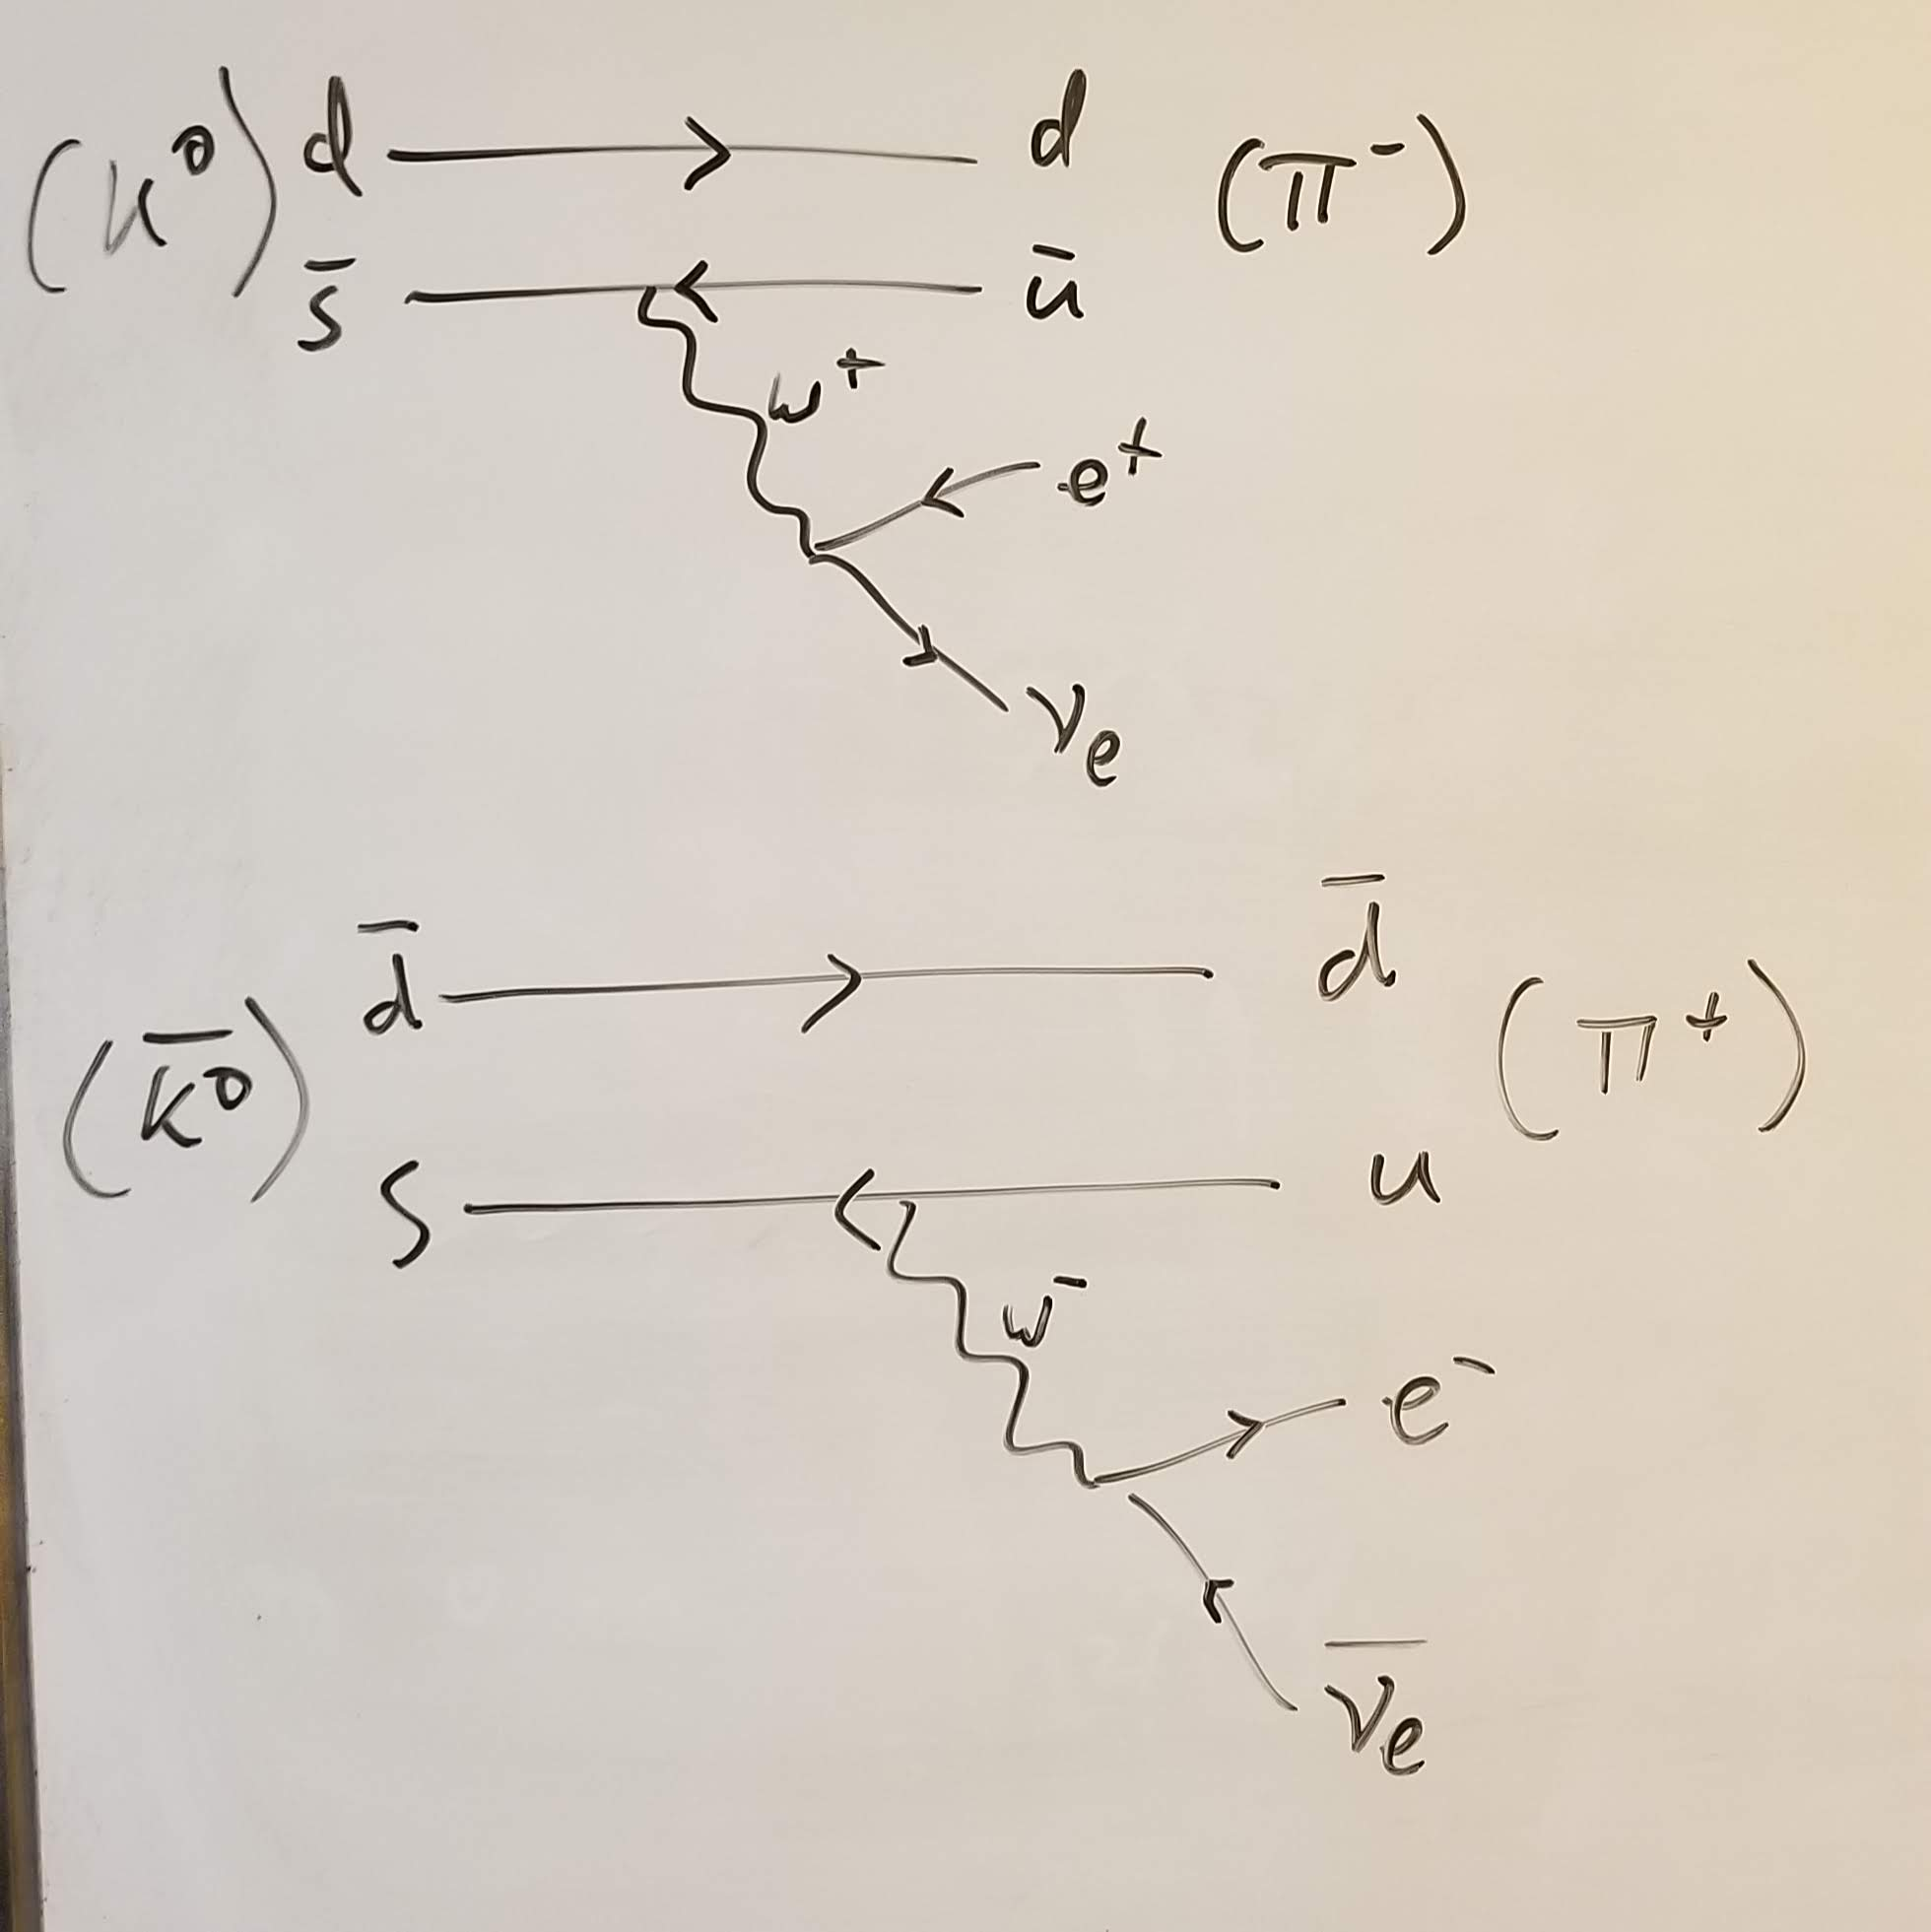
\includegraphics[scale=0.2]{kaons}
		\centering
		\caption{The two neutral kaon decays}
		\label{kaons}
		\centering
	\end{figure}
	
	\[
		\begin{split}
		\Gamma(K_L \rightarrow \pi^+e^-\bar{\nu}_e) \propto \abs{\braket{\bar{K}^0|K_L}}^2 \propto \abs{1-\epsilon}^2=(1-\epsilon)(1-\epsilon^*)=1-\epsilon^*-\epsilon+\abs{\epsilon}^2 \approx 1-2Re(\epsilon) \\ 
		\Gamma(K_L \rightarrow \pi^-e^+\nu_e) \propto \abs{\braket{K^0|K_L}}^2 \propto \abs{1+\epsilon}^2=(1+\epsilon)(1+\epsilon^*)=1+\epsilon^*+\epsilon+\abs{\epsilon}^2 \approx 1+2Re(\epsilon)
		\end{split}
	\]
	Here I dropped the $\epsilon^2$ term since we are only looking to first order in $\epsilon$. I also dropped any common constants since they will be the same for each term and will divide out in the end.
	\[
		\begin{split}
		\frac{\Gamma(K_L \rightarrow \pi^-e^+\nu_e)-\Gamma(K_L \rightarrow \pi^+e^-\bar{\nu}_e))}{\Gamma(K_L \rightarrow \pi^-e^+\nu_e)+\Gamma(K_L \rightarrow \pi^+e^-\bar{\nu}_e))} =& \frac{1+2Re(\epsilon)-(1-2Re(\epsilon))}{1+2Re(\epsilon)+(1-2Re(\epsilon))}\\
		=&\frac{4Re(\epsilon)}{2} = 2Re(\epsilon)
		\end{split}
	\]
	
\end{homeworkProblem}

\pagebreak

\begin{homeworkProblem}
	Defining
	\[
		\eta_{\pm}=\abs{\eta_\pm}e^{i\phi_\pm}=\frac{\braket{\pi^+\pi^-|K_L}}{\braket{\pi^+\pi^-|K_S}}
	\]
	calculate the probabilities of $\pi^+\pi^-$ decay as a function of proper time for an initial $K^0$ or $\bar{K^0}$ produced at $t=0$. Express your answer, up to common proportionality constants, in terms of $\epsilon,\abs{\eta_\pm},\phi_\pm,\Delta m, \Gamma_S,$ and $\Gamma_L$, where $\Delta m = K_S - K_L$. Keep only leading terms in $\epsilon$. Using the experimental values for these quantities, plot the two probabilities as a function of time in units of the $K_S$ lifetime, going out to 30 $K_S$ lifetimes.	
	\\
	\\
	\textbf{Solution}
	\\
	\\
	Here are the definitions of $K_L$ and $K_S$ in terms of $K^0$ and $\bar{K^0}$:
	\[
		\begin{split}
		\ket{K_L}=\frac{1}{\sqrt{1+\abs{\epsilon}}}\left[\frac{1+\epsilon}{\sqrt{2}}\ket{K^0}-\frac{1-\epsilon}{\sqrt{2}}\ket{\bar{K^0}}\right] \\
		\ket{K_S}=\frac{1}{\sqrt{1+\abs{\epsilon}}}\left[\frac{1+\epsilon}{\sqrt{2}}\ket{K^0}+\frac{1-\epsilon}{\sqrt{2}}\ket{\bar{K^0}}\right] 
		\end{split}	
	\]

	And here they are in terms of the CP eigenstates:
	\[
		\begin{split}
		\ket{K_L}=\frac{1}{\sqrt{1+\abs{\epsilon}}}\left[\ket{K_2}+\epsilon \ket{K_1}\right] \\
		\ket{K_S}=\frac{1}{\sqrt{1+\abs{\epsilon}}}\left[\ket{K_1}+\epsilon \ket{K_2}\right] 
		\end{split}
	\]
	First, define the time-evolution of the wave function in the same way it was done in the lecture notes: 
	\[
		\begin{split}
		\ket{K_S(t)}=&\ket{K_S}e^{im_St-\Gamma_St/2} \\
		\ket{K_L(t)}=&\ket{K_L}e^{im_Lt-\Gamma_Lt/2} \\
		\end{split}
	\]
		
	Here I will write the total wave function as a function of time but in the CP basis since we know that the $\pi^+\pi^-$ system is a CP eigenstate with an eigenvalue of +1. This will be helpful because we know the eigenvalues of $\ket{K_1}$ and $\ket{K_2}$
	\[
		\begin{split}
		\ket{\psi_{K^0}(t)}=& \frac{1}{\sqrt{2}}\left[\ket{K_S(t)} + \ket{K_L(t)} \right] \\
		=& \frac{1}{\sqrt{2}}\left[\ket{K_S}e^{im_St-\Gamma_St/2} + \ket{K_L}e^{im_Lt-\Gamma_Lt/2}\right] \\
		\ket{\psi_{\bar{K^0}}(t)}=& \frac{1}{\sqrt{2}}\left[\ket{K_S}e^{im_St-\Gamma_St/2} - \ket{K_L}e^{im_Lt-\Gamma_Lt/2}\right] \\
		\ket{\psi_{K^0}(t)}=&\frac{1}{\sqrt{2}}\frac{1}{\sqrt{1+\abs{\epsilon}}}\left[  (\ket{K_1}+\epsilon \ket{K_2})e^{im_St-\Gamma_St/2} + (\ket{K_2}+\epsilon\ket{K_1})e^{im_Lt-\Gamma_Lt/2}\right] \\
		=& \frac{1}{\sqrt{2}}\frac{1}{\sqrt{1+\abs{\epsilon}}}\left[ (e^{im_St-\Gamma_St/2}+\epsilon e^{im_Lt-\Gamma_Lt/2})\ket{K_1}+(e^{im_Lt-\Gamma_Lt/2}+\epsilon e^{im_St-\Gamma_St/2})\ket{K_2}\right] \\
		\ket{\psi_{\bar{K^0}}(t)}=& \frac{1}{\sqrt{2}}\frac{1}{\sqrt{1+\abs{\epsilon}}}\left[ (e^{im_St-\Gamma_St/2}-\epsilon e^{im_Lt-\Gamma_Lt/2})\ket{K_1}+(-e^{im_Lt-\Gamma_Lt/2}+\epsilon e^{im_St-\Gamma_St/2})\ket{K_2}\right]
		\end{split}
	\] 
	The subscript on the wave function state refers to the initial beam being either purely $K^0$ or purely $\bar{K^0}$.
	\\
	\\
	The probability to find the system in the state $\ket{\pi^+\pi^-}$ can be found like this:
	\[
		\begin{split}
		\abs{\braket{K_1|\psi_{K^0}(t)}}^2=&\frac{1}{2+2\abs{\epsilon}}\left[ (e^{im_St-\Gamma_St/2}+\epsilon e^{im_Lt-\Gamma_Lt/2})(e^{im_St-\Gamma_St/2}+\epsilon e^{im_Lt-\Gamma_Lt/2})^*\right] \\
		=& \frac{1}{2+2\abs{\epsilon}}\left[ e^{-\Gamma_St} +\abs{\epsilon}^2e^{-\Gamma_Lt} +\epsilon^*e^{i(m_S-m_L)t}e^{-(\Gamma_S+\Gamma_L)t/2}+\epsilon e^{-i(m_S-m_L)t}e^{-(\Gamma_S+\Gamma_L)t/2}\right] \\
		\approx& \frac{1}{2+2\abs{\epsilon}}\left[ e^{-\Gamma_St}+2Re(\epsilon e^{i\Delta mt}e^{-(\Gamma_S+\Gamma_L)t/2})    \right] \\
		\abs{\braket{K_1|\psi_{\bar{K^0}}(t)}}^2\approx&\frac{1}{2+2\abs{\epsilon}} \left[ e^{-\Gamma_St}-2Re(\epsilon e^{i\Delta mt}e^{-(\Gamma_S+\Gamma_L)t/2})    \right]
		\end{split}
	\]
	The plot of the probabilities can be found in Figure \ref{kaonlifetime}.
	
	\begin{figure}[h]
		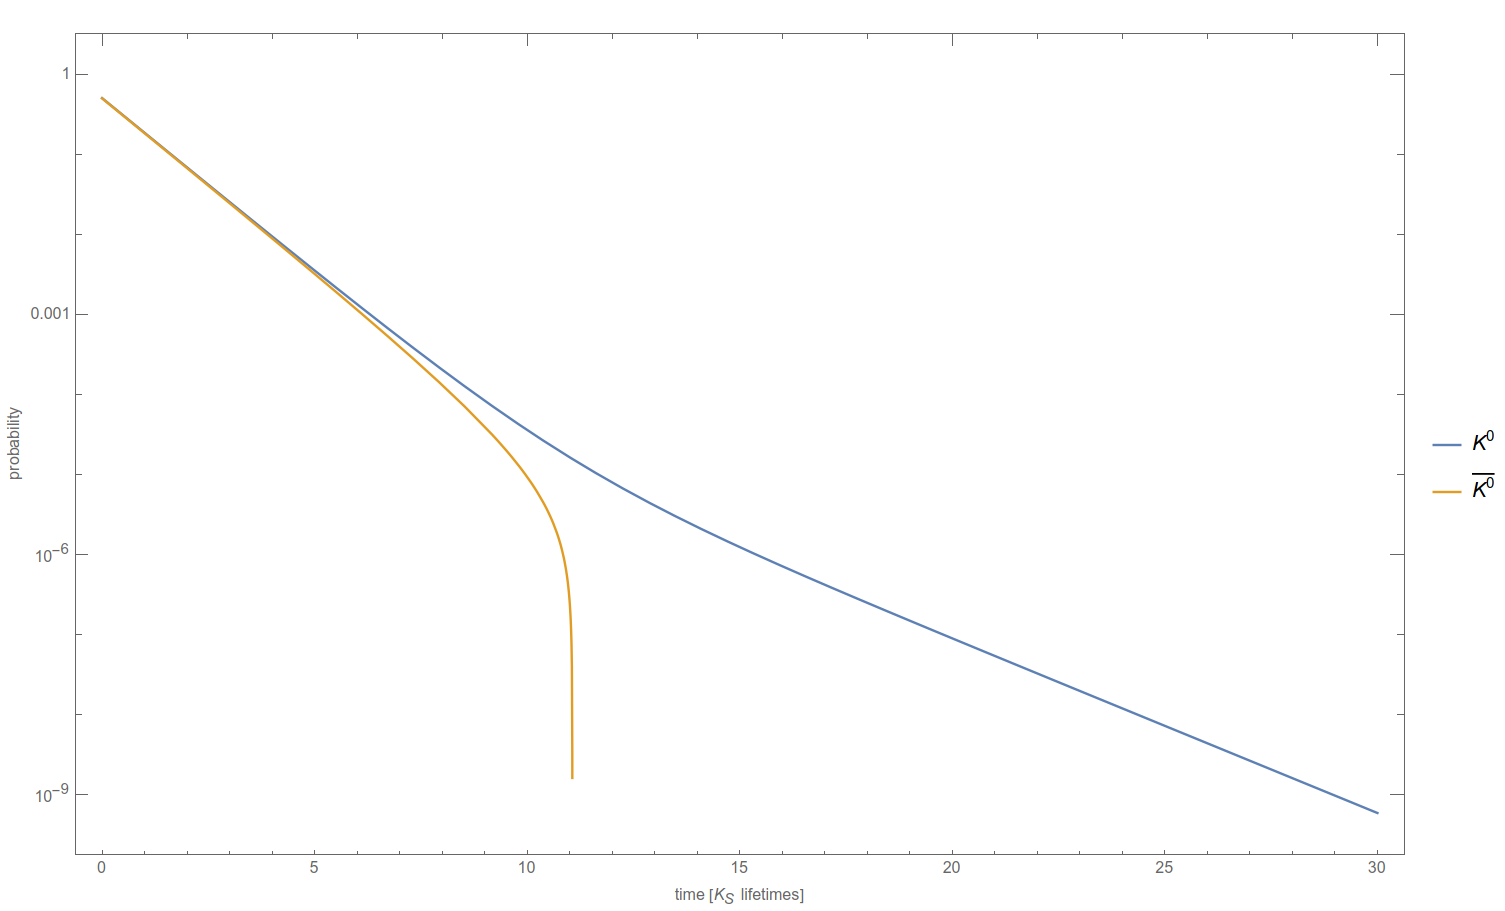
\includegraphics[scale=0.4]{kaonlifetime}
		\centering
		\caption{Probability for $K^0$ and $\bar{K^0}$ to decay to $\pi^+\pi^-$ as a function of $K_S$ lifetime. }
		\label{kaonlifetime}
		\centering
	\end{figure}
	
	
	
\end{homeworkProblem}

\pagebreak

\begin{homeworkProblem}
	Calculate $P(A,t;B)$, where $A$ and $B$ are either $K^0$ or $\bar{K^0}$. This is defined to be the probability that a neutral kaon in state $B$ at $t=0$ has oscillated into a state $A$ after a time $t$. Express your answer in terms of $\epsilon, \Delta m, \Gamma_S,$ and $\Gamma_L$. Keep only leading terms in $\epsilon$. Plot the probabilities as before, going out to 20 $K_S$ lifetimes, and using a factor of $\epsilon$ which is a factor of ten larger than the experimental value.
	\\
	\\
	\textbf{Solution}
	\\
	\\
	Once again, here are $K_L$ and $K_S$:
	\[
		\begin{split}
		\ket{K_L}=\frac{1}{\sqrt{1+\abs{\epsilon}}}\left[\frac{1+\epsilon}{\sqrt{2}}\ket{K^0}-\frac{1-\epsilon}{\sqrt{2}}\ket{\bar{K^0}}\right] \\
		\ket{K_S}=\frac{1}{\sqrt{1+\abs{\epsilon}}}\left[\frac{1+\epsilon}{\sqrt{2}}\ket{K^0}+\frac{1-\epsilon}{\sqrt{2}}\ket{\bar{K^0}}\right]
		\end{split}
	\]
	We can use these equations to write $K^0$ and $\bar{K^0}$ in terms of $K_L$ and $K_S$.
	\[
		\begin{split}
		\ket{K^0} =& \sqrt{\frac{1+\abs{\epsilon^2}}{2}}\frac{1}{1+\epsilon}\left[ \ket{K_L}+\ket{K_S} \right] \\
		\ket{\bar{K^0}} =& \sqrt{\frac{1+\abs{\epsilon^2}}{2}}\frac{1}{1-\epsilon}\left[ \ket{K_L}-\ket{K_S} \right]
		\end{split}
	\]
	Now write the wave functions with time included.
	\[
		\begin{split}
		\ket{K^0(t)} =& \sqrt{\frac{1+\abs{\epsilon^2}}{2}}\frac{1}{1+\epsilon} \left[e^{im_Lt-\Gamma_Lt/2}\ket{K_L} + e^{im_St-\Gamma_St/2}\ket{K_S} \right] \\
		\ket{\bar{K^0}(t)} =& \sqrt{\frac{1+\abs{\epsilon^2}}{2}}\frac{1}{1-\epsilon} \left[e^{im_Lt-\Gamma_Lt/2}\ket{K_L} - e^{im_St-\Gamma_St/2}\ket{K_S} \right]
		\end{split}
	\]
	Let's find the probability that a neutral kaon, $K^0$, at $t=0$ decays into its anti-particle, $\bar{K^0}$ at time $t$.
	\[
		\begin{split}
		\abs{\braket{K^0(t=0)|\bar{K^0}(t)}}^2 =& \abs{ \frac{1+\abs{\epsilon^2}}{2}\frac{1}{\abs{1+\epsilon}^2} \left[\bra{K_L} + \bra{K_S} \right]\left[e^{im_Lt-\Gamma_Lt/2}\ket{K_L} - e^{im_St-\Gamma_St/2}\ket{K_S} \right] }^2\\
		=&\left(\frac{1+\abs{\epsilon^2}}{2}\frac{1}{\abs{1+\epsilon}^2}\right)^2 \abs{\left[e^{im_Lt-\Gamma_Lt/2} - e^{im_St-\Gamma_St/2} \right] }^2 \\
		\approx&\frac{1}{4(1+4Re[\epsilon])}\left[ e^{-\Gamma_Lt}+e^{-\Gamma_St} + 2Re\left( e^{-i\Delta mt}e^{-(\Gamma_S+\Gamma_L)t/2}\right) \right]
		\end{split}
	\] 
	Between the second and third lines, I dropped all factors of $\epsilon$ which were of order greater than 1. You will find the plot of this probability in Figure \ref{kaonoscillation}. 
	\\
	\\
	If you start with a particle in state $\bar{K^0}$ going to $K^0$, you will get the same plot. The only difference in the equation will be in the prefactor you will have a $1-4Re(\epsilon)$ instead of $1+4Re(\epsilon)$ in the denominator, but because $\epsilon$ is so small, the difference will be negligible.
	\begin{figure}[h]
		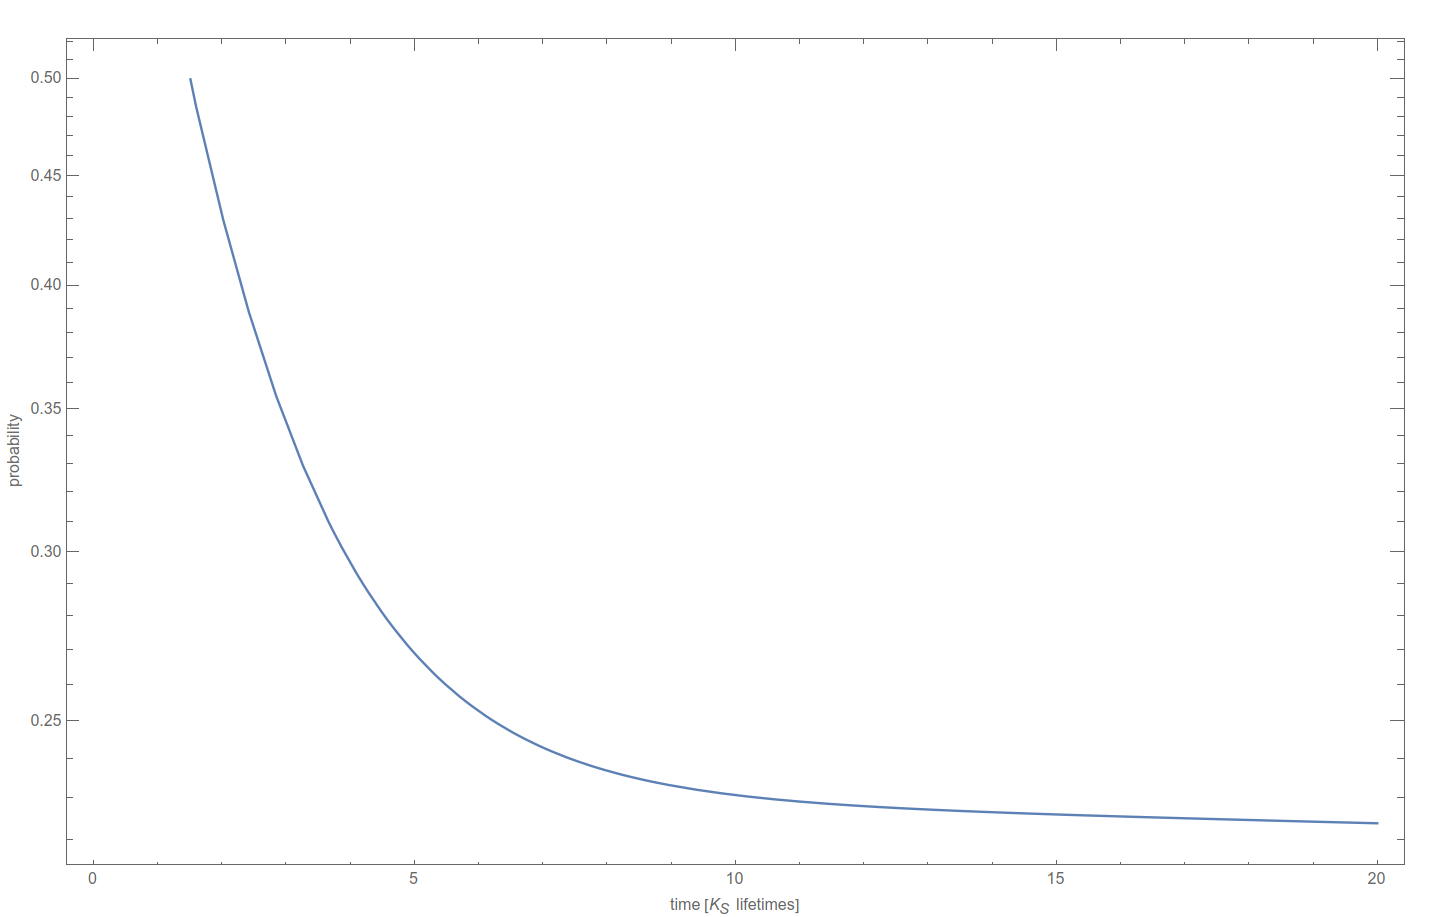
\includegraphics[scale=0.4]{kaonoscillation}
		\centering
		\caption{Probability for $K^0$ to oscillate to $\bar{K^0}$ as a function of time}
		\label{kaonoscillation}
		\centering
	\end{figure}
\end{homeworkProblem}

\pagebreak

\begin{homeworkProblem}
In class we briefly mentioned the (approximate) $\Delta I = 1/2$ rule, which says that in strange particle decays, transitions with $\Delta I = 1/2$ are enhanced over those with $\Delta I = 3/2$. Use this rule to derive:
\[
	\Gamma(K_L \rightarrow 3\pi^0)=\frac{3}{2}\Gamma(K_L\rightarrow \pi^+\pi^-\pi^0)
\]
and compare this result with experimental data. Make the reasonable assumption that all pairs of pions are in an $L=0$ state. Don't forget that pions are bosons and you'll need to write totally symmetric wave functions.
\\
\\
\textbf{Solution}
\\
\\
\end{homeworkProblem}

\end{document}

